\documentclass[aps,prb,twocolumn,showpacs,superscriptaddress]{revtex4-2}
%\documentclass[aps,prb,showpacs,twocolumn,amsmath,amssymb,superscriptaddress]{revtex4-2}
\bibliographystyle{apsrev4-2}

\usepackage{tabularx}
\usepackage{bm}
\usepackage{bookmark}
%\usepackage[demo]{graphicx}
\usepackage{graphicx}
\usepackage{tikz}
%\usepackage{setspace}
%\setstretch{3}

\usepackage{hyperref}
\hypersetup{colorlinks=true,urlcolor= blue,citecolor=blue,linkcolor= blue,bookmarks=true,bookmarksopen=false}

\usepackage{color}

\usepackage{amsmath,mathtools}
\usepackage{multirow}
\usepackage{dcolumn}
\usepackage{amssymb,amscd,xypic,bm,wasysym}
\usepackage{float}
\usepackage{cleveref}
\usepackage[caption=false,position=top,captionskip=0pt,farskip=0pt]{subfig}
\captionsetup[subfigure]{justification=raggedright,singlelinecheck=false}

\newcommand{\Red}[1]{\textcolor{red}{#1}}
\newcommand{\Blue}[1]{\textcolor{blue}{#1}}
%\newcommand{\vb}[1]{\boldsymbol{#1}}
\usepackage{soul}

% reset vec and hat style to a bold type
\let\oldhat\hat
\renewcommand{\hat}[1]{\oldhat{\mathbf{#1}}}
\renewcommand{\vec}[1]{\mathbf{#1}}
% stretches the vertical spacing of arrays/matrices
\renewcommand{\arraystretch}{1.5}
\setlength{\jot}{10pt}

\newcommand{\ham}{\mathcal{H}}
\newcommand{\cc}{c^{\dagger}}
\newcommand{\de}{\Delta}

\begin{document}

\title{Landau Level-like Topological Floquet Hamiltonians}

\author{Aidan Winblad}
\affiliation{Department of Physics, Colorado State University, Fort Collins, CO 80523, USA}

\author{M. Tahir}
\affiliation{Department of Physics, Colorado State University, Fort Collins, CO 80523, USA}

\author{Hua Chen}
\affiliation{Department of Physics, Colorado State University, Fort Collins, CO 80523, USA}
\affiliation{School of Advanced Materials Discovery, Colorado State University, Fort Collins, CO 80523, USA}

\begin{abstract}
Motivated by the recent discovery of Floquet systems, we demonstrate that these produce an unconventional form of quantized Landau Level-like spectrum and the corresponding quantum Hall effect without need of an external perpendicular magnetic field.
The unconventional quantization in Floquet systems is caused by employing two linearly polarized laser lights in the off-resonant regime with one light being spatially inhomogeneous.
This notably distinguishes Landau levels in nonequilibrium Floquet systems from conventional quantum Hall effects observed in equilibrium under the application of strong magnetic field.
These results exhibit the fundamental question of realizing quantum Hall effect in nonequilibrium systems and point to a new direction for nano-electronic devices.
We elucidate the origin of the quantized Hall conductance and the Berry phase by using the Floquet theory--adiabatic trajectory of wave packets.
\end{abstract}

\maketitle

\emph{Introduction.---} The quantum Hall effect (QHE) in conventional two-dimensional electron gas (2DEG) is one of the most remarkable phenomena in condensed matter physics \cite{QHE1}.
This effect arises when a uniform external perpendicular magnetic field quantizes the electron energy spectrum into discrete Landau levels (LLs).
Subject to a strong magnetic field, the diagonal (longitudinal) electric conductivity is vanishingly small, while the nondiagonal (Hall) conductivity is quantized.
This happens when the Fermi energy lies in the gap between two LLs, referred to as integer QHE as the Hall conductivity takes values of $-Ce^2/h$ with integer $C$, being the number of occupied bands below the Fermi energy \cite{QHE4}.
Recent experimental realization of graphene has stimulated additional interest to explore QHE in two dimensional systems \cite{QHE2, QHE3, QHE4}.
%Graphene exhibits unusual quantized Hall conductivity values of $2(2n + 1)e^2/h$ due to application of the magnetic field \cite{QHE4}, which are different from conventional 2DEG.

This significant effect is important to explore in Floquet systems \cite{NHL, AEE} because one may observe new phases in an alternative venue that can be experimentally realized \cite{MCR, YHW, HZJ, JWM,merboldtObservationFloquetStates2024, choiDirectObservationFloquetBloch2025}.
Time periodically modulated Floquet theory has been extensively studied and well established for a large class of systems \cite{JHS,HSA,MGP,MBL,AEE,NGJ}.
One can then employ the high frequency expansions \cite{MBL,AEE,NGJ,SRI,API,TMS,ESM,TKT,ALA} such as the well known Floquet-Magnus expansion \cite{ESM,TKT,ALA,FCA} and Van Vleck expansion \cite{MBL,AEE}, to analyze these effects.
The significant difference is the latter provides an explicit formula for the time evolution operator starting at initial time $t_{0}=0$ rather than former starting with finite time $t_{0}$ \cite{supp}.
In nonequilibrium systems, circularly polarized laser light can drive transitions that induce nontrivial topological phases, even in materials that are topologically trivial in equilibrium \cite{TKO}.
%This mechanism for nonequilibrium physics resembles quantum Anomalous Hall effect proposed by Haldane \cite{Haldane} in equilibrium systems.

Optical manipulation of electronic properties has been emerging as a promising way of exploring novel phases \cite{AKA, JHM}.
This leads to Floquet-Bloch states exhibiting emerging physical properties that are otherwise inaccessible in equilibrium \cite{LST}.
Examples include Floquet Chern insulator \cite{AGG}, Floquet topological insulators \cite{rudnerBandStructureEngineering2020}, Floquet notion of magnetic and other strongly-correlated phases\cite{rudnerBandStructureEngineering2020}, manipulation of topological antiferromagnet \cite{bielinskiFloquetBlochManipulation2025}, topological classifications, symmetry-breaking concept, and symmetry protected topological phases in nonequilibrium quantum many-body systems \cite{EKM, rudnerBandStructureEngineering2020}.
However, it is important to note that these studies have been demonstrated in the presence of time-periodic homogeneous laser lights.
The role of spatially inhomogeneous laser light \cite{SWP1, SWP2, SWP3, SWP4, SWP5} remains largely unexplored.

In this work, we demonstrate that QHE can be observed in Floquet systems without need of a uniform magnetic field.
We show that three linearly polarized lights are an effective and versatile way of realizing QHE, both in graphene-like 2D systems or in conventional 2DEGs.
Additionally, two of the lights need to be spatially inhomogeneous and mirror one another to create a standing wave on the material.
Employing Floquet theory, we rely on the standard degenerate perturbation formalism and use the Van Vleck expansion \cite{MBL, AEE} to derive an effective Hamiltonian and corresponding bandstructure in the long wavelength limit.
We leverage high-refractive index materials \cite{shimFundamentalLimitsRefractive2021} to enhance the effective magnetic fields and energy bandstructure.
Our work provides new platforms for realizing QHE and related novel phases in nonequilibrium systems.

\emph{Floquet Landau level-like bands in Dirac systems.---} In this section we demonstrate a Dirac system in the presence of a standing, non-uniform, circularly polarized light becomes an effective Dirac Hamiltonian with a magnetic field that is composed of the electric field component of light.
Dirac electrons can be represented with a generic model 2D Hamiltonian honeycomb monolayer in the presence of a gauge potential as

\begin{figure}[h]
  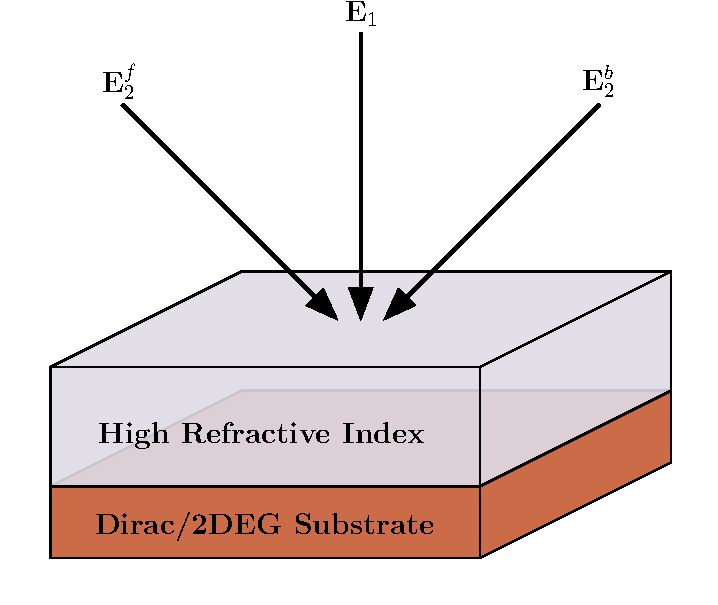
\includegraphics[width=0.4\textwidth]{./figures/fll-setup.pdf}
  \caption{Schematic of two oblique (forward and backward) and one normally incident light on graphene or a 2DEG substrate with high refractive index material on top. Oblique lasers have polarization in $y$-axis and travel in $xz$-plane and normally incident laser has polarization in the $x$-axis and travel in $yz$-plane. With beam width large enough to cover the device fully.}
  \label{fig:fll-setup}
\end{figure}

\begin{equation}\label{eq:HDirac}
  \ham(t) = v_{F} \bm{\sigma} \cdot \left(\vec{p} + e\vec{A}(t)\right),
\end{equation}
where $\vec{A}$ is the gauge potential, $\vec{p}$ is the momentum operator, $v_F$ is the Fermi velocity of Dirac fermions, $e$ is electron charge, and $\vec{\sigma}$ the Pauli matrices vector in 2D.
The light is made of three linearly polarized lasers, as shown in Fig. \ref{fig:fll-setup}.
Where the first is normally incident in the $z$-axis with polarization in the $x$-axis.
The second and third are of oblique incidence in the $xz$-plane, to acquire non-uniformity in the $x$-axis, with polarization in the $y$-axis, and mirrored about the $yz$-plane.
This is to introduce $x$-dependence with the $p_y$ term of the Dirac Hamiltonian.
The relevant electric field components at the Dirac system interface are

\begin{align} \label{eq:EDfield}
\vec{E}_{1} &= E\cos \omega t\ \hat{x}, \nonumber \\
\vec{E}_{2} &= \vec{E}_2^f + \vec{E}_2^b = E\sin(Kx)\sin 2\omega t\ \hat{y},
\end{align}
%Where $\omega$ is angular frequency of light with time $t$ and $K=2\pi /d$ with $d$ being the spatial period of the electric field with amplitude $E$.
Where $\omega$ is angular frequency of the laser with time $t$ and $K = \omega \sin{(\theta_i)} / v_p$, with $\theta_i$ as incident angle of the oblique lasers and $v_p$ is phase velocity of the lasers.
%Notice, the second electric field has twice frequency of the first, this is a requirement to make the Dirac Hamiltonian into a Landau level-like Hamiltonian, the derivation in REFERENCE APPENDIX can inform the reader of this choice.
Notice, the second electric field has twice frequency of the first, this allows for the second gauge potentials $\sigma_y$ to have non-zero commutation with the first gauge potentials $\sigma_x$, and due to the high-frequency expansion used later, allows for the second gauge potential to return to a $\sigma_y$, as seen in \ref{fll-dirac-derivation}.
This form of the electric field relates to the following gauge potential, via $\vec{E} = -\partial_t \vec{A}$ as

\begin{equation}\label{eq:ADirac}
  \vec{A}(t)= \dfrac{E}{\omega} \left\langle -\sin \omega t, \tfrac{1}{2}\sin(Kx) \cos 2\omega t \right\rangle,
\end{equation}%
Substituting Eq.~\eqref{eq:ADirac} into Eq.~\eqref{eq:HDirac}, we arrive at%

\begin{equation}\label{eq:HDtime}
  \ham(t)= v_{F}\bm{\sigma}\cdot\vec{p} - \sigma _{x} \dfrac{v_F eE}{\omega} \sin {\omega t} - \sigma _{y} \dfrac{v_F eE}{2\omega}\sin{(Kx)} \cos2\omega t.
\end{equation}%
Due to the laser's time-translation symmetry through $A(t+T)=A(t)$ with $T=2\pi /\omega $, one can apply the Floquet theory \cite{AEE, MBL, supp} and obtain an effective Hamiltonian from Eq.~\eqref{eq:HDtime}.
This introduces the quasienergy matrix $Q_{m,m+n} = H_n + m\hbar\omega\delta_{n0}$ after performing the Fourier time-transform of the Hamiltonian, given as

\begin{equation} \label{eq:fourier-time-transform}
  H_n = \dfrac{1}{T} \int_{0}^{T} \ham(t) e^{-in\omega t} dt,
\end{equation}
then we are left with modes $m=0,\pm1,\pm2$.
To use the high-frequency approximation we require $\hbar\omega \gg H_{\pm1,\pm2}$, the off-diagonal terms.
After applying the high-frequency approximation to first and second order expansion in $\hbar\omega$, it leads to the zeroth-mode effective Hamiltonian in Eq.~\eqref{eq:HDtime} as

\begin{align} \label{eq:HDeff}
  H_{\text{eff}}= &v_{F}\bm{\sigma}\cdot\vec{p}-\sigma_y\frac{v_F^3 e^2 E^2 p_y}{\hbar^{2}\omega^{4}}
  +\sigma_y\frac{v_F^3 e^3 E^{3}\sin{(Kx)}}{4\hbar^{2}\omega^{5}} \nonumber \\
  &-\sigma_x\frac{v_F^3 e^2 E^2 \left\{p_x, \sin^2{(Kx)} \right\} }{8\hbar^{2}\omega^{4}}.
\end{align}
The derivation can be found in the Appendix \ref{fll-dirac-derivation}.
This effective Hamiltonian can be simplified in the long wavelength limit, $Kx \ll 1$ to

\begin{align} \label{eq:HeffDirac}
  %\ham_{\text{eff}} &= v_F \sigma_x p_x + v_F \sigma_y \left[ \left( 1- \dfrac{v_F^2e^2E^2}{\hbar^2\omega^4} \right) p_y + \dfrac{K v_F^2 e^3 E^3}{4 \hbar^2 \omega^5} x \right] \nonumber \\
  \ham_{\text{eff}}^D &= v_{F}\sigma_{x}p_{x}+v_F\sigma_{y} \left( C p_{y} + eB^Dx \right),
\end{align}%
where $C = 1-\left(\tfrac{v_{F}eE}{\hbar\omega^2}\right)^2$ and $B^D=\frac{Kv_F^2 e^2E^3}{4\hbar^{2}\omega^{5}}$.
%In accordance with Eqs.~\eqref{eq:HDeff} and ~\eqref{eq:HeffDirac}, there is least anisotropy in the Dirac spectrum in addition to zero gap.
Diagonalizing the Hamiltonian in Eq.~\eqref{eq:HeffDirac}, we obtained the eigenvalues for Dirac system as%

\begin{equation} \label{eq:DiracEner}
  \epsilon_{n}^D = \pm v_F^2 \sqrt{\dfrac{nK e^3 E^3}{2 \hbar \omega^5}}
\end{equation}
which is similar to graphene LLs spectrum in the limit of equal velocities.
The effective magnetic field in the Dirac Hamiltonian achieves a highly degenerate energy spectrum similar to LLs.
Unlike conventional LLs, the electron motion is not a cyclotron orbit but a potentially more complicated orbit, due to CPL inducing a Coulumb force in the material's 2D plane.
In Eq. ~\eqref{eq:HDeff}, the first order term in $\hbar \omega$ leads to gap at the Dirac point in normally incident, circularly polarized light experiments \cite{YHW, JWM} and is zero here due to the non-uniformity nature of oblique incident lasers.

There are several ways to enhance the effective magnetic field and directly LL-like energies for a Dirac system.
Electric field strength can be increased within reason as we are limited by the photon energy to ensure the high-frequency expansion holds, $E \ll 2\hbar\omega^2/e v_F$.
One can reasonably use electric field strengths up to 20\% of the limit due to photon energy.
The laser wavenumber $K= \omega \sin{(\theta_i)} / v_p$ has a linear relationship to photon energy, too.
Overall, considering the high-frequency limit on the electric field, the effective field $B^D \propto \omega^2 \sin{(\theta_i)} / (v_F v_p)$.
Without too much consequence, the incident angle can be increased up to $\pi/2$ and decreasing the phase velocity of light would enhance the effective magnetic field.
Increasing photon energy is one way to enhance the effective magnetic field.
As considered in previous literature, when photon energy and electric field are increased more energy is pumped into the system, shorter pulses are required to prevent damaging the system \cite{YHW, JWM}.

\emph{Floquet Landau level-like bands in 2DEG systems.---} In this section we show a 2DEG system with a standing, non-uniform, circularly polarized light becomes an effective 2DEG Hamiltonian with an effective magnetic field composed of the electric field component of light.
We consider the case of Schr\"{o}dinger charged particles in the presence of a gauge potential as
\begin{equation}\label{eq:H2deg}
  \ham(t) = \dfrac{1}{2m^*} \left( \vec{p} + e \vec{A}(t)\right)^2
\end{equation}
where $m^*$ is the effective charge mass.
We again consider a similar setup with three linearly polarized lasers.
The relevant electric field components at the 2DEG interface are
\begin{align} \label{eq:E2field}
  \vec{E}_{1} &= E \cos{\omega t}\ \hat{x}, \nonumber \\
  \vec{E}_{2} &= \vec{E}_2^f + \vec{E}_2^b = -E\cos{(K x)} \sin{\omega t}\ \hat{y}.
\end{align}%
Unlike the Dirac system, all lasers have them same frequency.
This ensures a LL-like behavior from the nonzero commutation of $x$ and $p_x$ terms during the high-frequency expansion.
The electric field relates to the following gauge potential, via $\vec{E} = -\partial_t \vec{A}$ as

\begin{equation}\label{eq:A2deg}
  \vec{A}(t)= \dfrac{E}{\omega} \left\langle -\sin \omega t, \cos{(Kx)} \cos{\omega t} \right\rangle.
\end{equation}%
Substituting Eq. \eqref{eq:A2deg} into Eq. \eqref{eq:H2deg}, we arrive at

\begin{align}\label{eq:H2time}
  \ham(t) = &\dfrac{p_x^2 + p_y^2}{2m^*} + \dfrac{e^2 E^2}{4m^* \omega^2}(1-\cos{2\omega t}) \nonumber \\
  &+ \dfrac{e^2 E^2}{4m^*\omega^2}(1+\cos{4m^* \omega t}) \cos^2{(Kx)} \nonumber \\
  &+\dfrac{2eE}{2m^* \omega} \left(p_y \cos{(Kx)}\cos{\omega t} -  p_x \sin{\omega t}\right).
\end{align}
Again, due to laser's time-translation symmetry we can apply the Floquet theory, which includes computing the Fourier time-transform using Eq. \eqref{eq:fourier-time-transform}.
This leaves us with modes $m=0,\pm1,\pm2$.
In the high-frequency expansion we still require $\hbar \omega \gg H_{\pm1,\pm2}$.
After applying the high-frequency approximation to first order in $\hbar \omega$, it leads to the zeroth-mode effective Hamiltonian as

\begin{align}\label{eq:H2eff}
  %\ham_{\text{eff}} &= \dfrac{1}{2m^*} \left[ p_x^2 + p_y^2 + \dfrac{e^2 E^2}{\omega^2}\left(1+\cos^2{(Kx)}\right) - \dfrac{2 K e^2 E^2 p_y \sin{(Kx)}}{m^*\omega^3} \right] \nonumber \\
  \ham_{\text{eff}} &= \dfrac{1}{2m^*} \Biggl[ p_x^2 + \left(p_y - \dfrac{K e^2 E^2 \sin{(Kx)}}{m^*\omega^3} \right)^2 \nonumber \\
  &+ \dfrac{e^2 E^2 \cos^2{(Kx)}}{\omega^2}  - \dfrac{K^2 e^4 E^4 \sin{(Kx)}}{m^{*2}\omega^6} \Biggr]. \nonumber
\end{align}
where we shifted a constant energy out of the effective Hamiltonian and completed the square for the $p_y$ and $x$ terms.
Here we can see the high-frequency expansion terms $H^{F(1)}$ and $H^{F(2)}$, introduces a periodic potential in the x-direction, this can be cancelled out by applying an external periodic potential of the same strength and wavenumber in the x-direction \cite{supp}.
Finally, in the long wavelength, $Kx \ll 1$,

\begin{equation}\label{eq:Heff2deg}
  \ham_{\text{eff}}^{\text{2DEG}} = \dfrac{1}{2m^*} \left[ p_x^2 + {\left(p_y - eB^{\text{2DEG}}x \right)}^2  \right],
\end{equation}
with $B^{\text{2DEG}} = \tfrac{K^2 e E^2 }{m^*\omega^3}$.
The energy spectrum values are
\begin{equation}\label{eq:2DEGenergy}
  \epsilon_n^{\text{2DEG}} = \dfrac{\hbar K^2 e^2 E^2}{m^{*2}\omega^3} \left(n+\dfrac{1}{2}\right),
\end{equation}
which is similar to 2DEG LLs spectrum.
This is another highly degenerate LL-like spectrum due to an effective magnetic field induced by the combination of lasers provided.

The 2DEG system has the same ways to enhance its effective magnetic field and energy spectrum.
First, the electric field is limited by the high-frequency expansion, we find $E \ll (8m^*\hbar\omega^3/e^2)^{1/2}$ to be a reasonable cutoff.
The effective field $B^{\text{2DEG}} \propto \omega^2 \sin^2{(\theta_i)} / v_p^2$, is similar to the Dirac system.
For a 2DEG system, the enhancement to the effective magnetic field follows a squared dependence on the incident angle and phase velocity, differing from the Dirac case, where it scales linearly and by Fermi velocity.
Similarly, increasing the photon energy is one way to enhance the effective magnetic field, with the requirement of using shorter pulses as photon energy and electric field increase.

\emph{Conclusion.---} We now examine the topology of both systems.
Eqs. \eqref{eq:HeffDirac} and \eqref{eq:Heff2deg} are in LL Hamiltonian form, and typically exhibit QHE.
The two systems only have translational symmetry in the $y$-axis, so a Chern number based on periodicity in $k_x$ and $k_y$ is not applicable, though one can relate the center of mass of an electron to the Chern number \cite{supp}, which is related to the Laughlin pump.
Considering the Laughlin pump argument, both systems have quantized Hall conductivity, since both have the same eigenstates as their respective LL Hamiltonian.
A key difference to note about both systems is the $C$ term in Eq. \eqref{eq:HeffDirac}.
This term will stay positive for the values of $E$ used in the high-frequency limit for the Dirac case.

Using existing experiments \cite{YHW, JWM} we can provide an estimate for the strength of the effective magnetic field to observe LL-like spectrum and QHE.
Analytical structure of Eq.~(\ref{eq:DiracEner}) and Eq.~(\ref{eq:2DEGenergy}) are primarily responsible for the LL-like spectrum in both the Dirac and 2DEG systems, respectively.
Although such results are valid for other 2D materials or Schr\"{o}dinger systems, however, for simplicity, we will consider parameters realized for graphene or topological insulators \cite{YHW, JWM}.
We will consider a similar range of mid-IR photon energies (or $\lambda = [3\mu $m$ , 10\mu $m$]$) as seen in graphene or topological insulators \cite{YHW, JWM} to match with recently proposed high refractive index metamaterial composites \cite{shimFundamentalLimitsRefractive2021}.
In these experiments \cite{YHW, JWM}, the strength of the electric field used is $1 \times 10^7$ V/m to $1 \times 10^8$ V/m, for the parameters used to estimate effective magnetic fields for both systems the largest electric field is around $1.4 \times 10^8$ V/m.
As should be considered, the larger both photon energy and electric field become ultrafast pulses should be used to prevent thermal damage to materials, on the order of $500$ fs.
To note, for the following results we assume a high oblique angle to let $\sin{(\theta_i)} \approx 1$.

To enhance the effective magnetic field, aside from using higher photon energy, reducing the photon phase velocity can see a considerable increase in both systems.
The refractive index materials can be set above graphene, or any Dirac material, such that the lasers can propagate through to reduce its phase velocity.
Germanium refractive index increases monotonically with increasing photon energy, we use a linear interpolation of the refractive index due the small change for the range of photon energies used.
Al-composite metamaterials refractive index is monotonically decreasing with increasing photon energy and we use a linear interpolation here as the data is roughly linear.

\begin{figure}[h]
  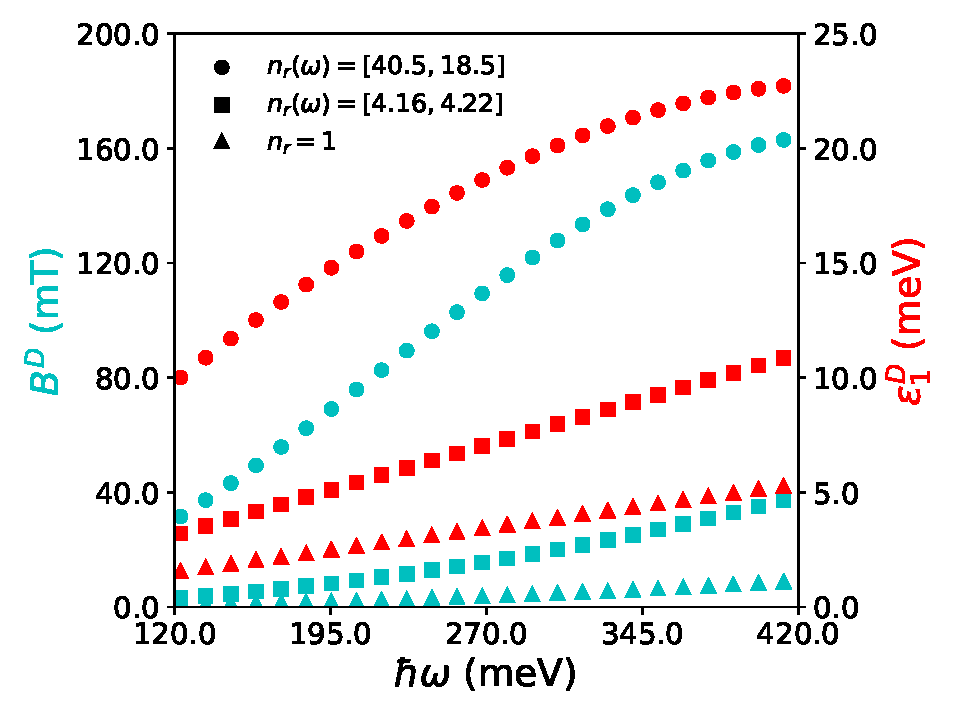
\includegraphics[width=0.45\textwidth]{./figures/dirac-eff-bfield-energy.pdf}
  \caption{Effective magnetic field (cyan) and first quasienergy (red) as a function of photon energy for various refractive materials: vacuum (triangles), germanium (squares), and  Al-composite metamaterial (circles).}
  \label{fig:dirac-bfield-energy}
\end{figure}

In case of a Dirac system Fig. \ref{fig:dirac-bfield-energy} shows graphene with various refractive index materials to enhance the effective magnetic field and first order quasienergy of the LL-like spectrum.
For mid-IR ranges of lasers, the effective magnetic field (cyan) can get up to $8.8$ mT for vacuum, $37.2$ mT for germanium, and $163$ mT for Al-composite metamaterial for $\hbar\omega=413$ meV and results in first order quasienergies (red) of $5.3$ meV, $11$ meV, and $23$ meV, respectively.
As can be seen in \ref{fig:dirac-bfield-energy} as photon energy increases the Al-composite refractive index decreases quite a bit and if we used higher energy we would see the effective magnetic field and quasienergies start to decrease, as will be seen with 2DEG.
While the material has higher index of refraction overall, it would be better to find a material that increases refractive index with photon energy, like germanium can, for it can drastically increase for slightly higher photon energies before effective magnetic field dips \cite{amotchkinaCharacterizationEbeamEvaporated2020}.

\begin{figure}[h]
  \subfloat[]{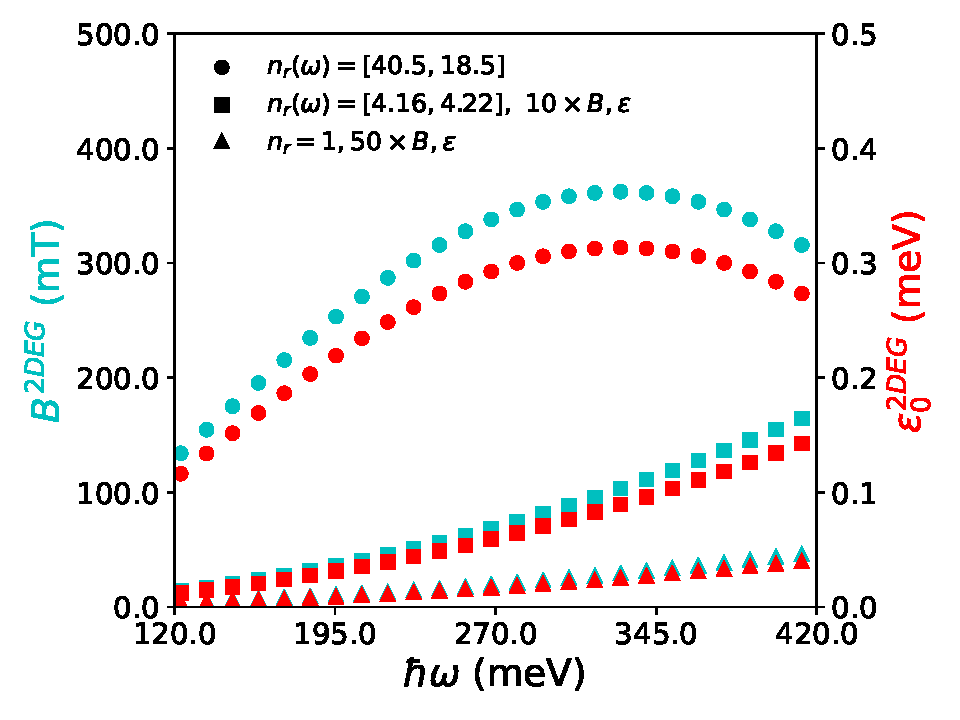
\includegraphics[width=0.45\textwidth]{./figures/2deg-eff-bfield-energy-GaAs.pdf}}\\
  \subfloat[]{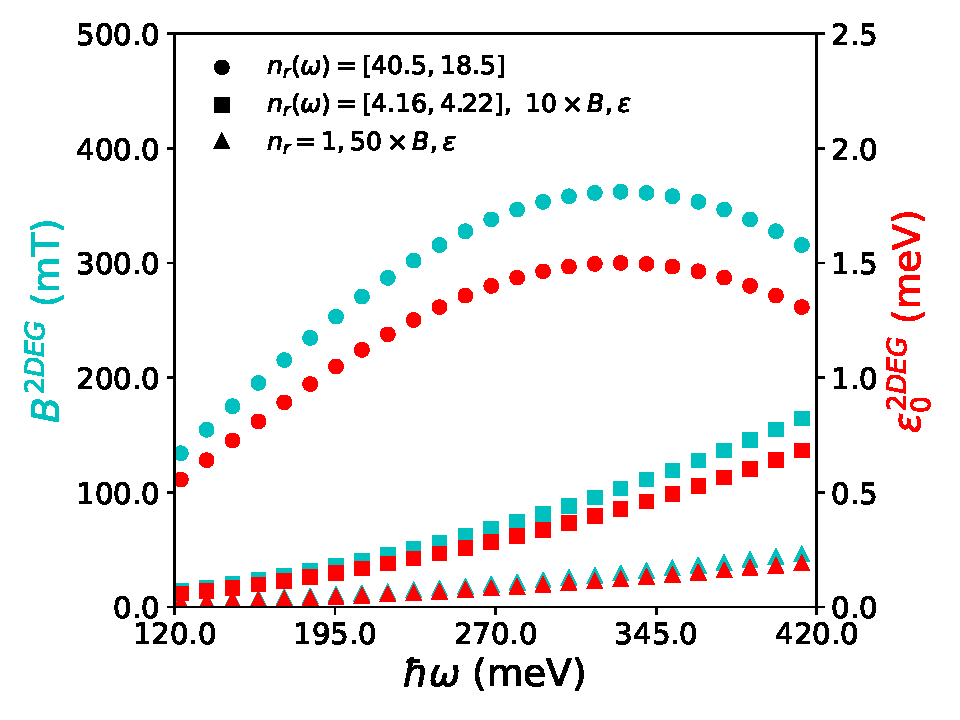
\includegraphics[width=0.45\textwidth]{./figures/2deg-eff-bfield-energy-InSb.pdf}}
  \caption{Effective magnetic field (cyan) and first quasienergy (red) as a function of photon energy for 2DEGs for various refractive materials: vacuum (triangles) scaled by a factor of 50, germanium (squares) scaled by a factor of 10, and Al-composite metamaterials. The 2DEG materials used are (a) GaAs and (b) InSb.}
  \label{fig:2deg-bfield-energy}
\end{figure}

For 2DEG systems Fig. \ref{fig:2deg-bfield-energy} shows GaAs and InSb materials with the same refractive materials used for graphene to enhance effective magnetic field and zeroth order quasienergy of the LL-like spectrum.
The vacuum and germanium interfaces are scaled up by a factor of $10$ and $50$, respectively, to visually enhance and compare it to the Al-composite interface.
GaAs is used as it is one of the most common 2DEG with relatively small effective electron mass, followed by InSb since it has the smallest effective electron mass found in 2DEG materials.
For the GaAs system, effective magnetic field (cyan) can get up to $0.92$ mT for vacuum, $16.5$ mT for germanium, and $362$ mT for Al-composite metamaterial and achieves zeroth order quasienergies (red) of $0.8\ \mu$eV, $14.3\ \mu$eV, and $314\ \mu$eV, respectively.
In the InSb system, effective magnetic field is the same as GaAs, since it has no dependence on effective mass, and achieves zeroth order quasienergies (red) of $3.8\ \mu$eV for vacuum, $68.2\ \mu$eV for germanium, and $1.5$ meV for Al-composite.
As alluded to earlier, due to Al-composites large decrease in refractive index for increasing photon energy, it peaks earlier around $\hbar\omega=328$ mT, for 2DEG.
Overall, we see large changes in 2DEG for both effective magnetic field, due to being proportional to refractive index squared and quasienergies, being inversely proportional to effective electron mass.

There are a few items we did not consider for our calculations.
First, we do not consider any effects due to a refractive index material in contact with a Dirac or 2DEG system.
Secondly, while the high-frequency expansion limits the electric field applied to the materials one could still go beyond the limit of $\hbar \omega \ll H_{\pm 1}, H_{\pm2}$ to enhance the effective magnetic field by a few orders of magnitude with some error.
For example, if instead we use $\hbar\omega = H_{\pm1}, H_{\pm2}$, this would be multiplying the electric field by a factor of $5$ from our calculations presented, Dirac effective magnetic field would increase by a factor of $125$ while 2DEG effective magnetic field would increase by a factor of $25$.
For Dirac systems with higher electric field strengths, if $C=0$, there would be no QHE as there is no coupling between $x$ and $p_y$, and if $C<0$, the direction of chirality reverses.

In conclusion, we have shown Floquet LLs and the QHE using three linearly polarized lasers, two of them mutually mirrored and having oblique incidence, for Dirac and conventional 2DEG systems.
We have presented results using a frequency space expansion method and degenerate Floquet perturbation theory.
A tight-binding model capable of using ``low-frequency'' with a Peierls substitution can be found in the supplemental material \cite{supp}, although these results are currently difficult to interpret.
Out paper's results indicate Floquet LL-like spectral features can appear in experimentally accessible parameters range.
Also, it is vital to note that we are flexible to use different values of the electric field strength, photon energy, or phase velocity to realize QHE and control the strength of the effective magnetic field.
Therefore, we predict Floquet LL-like spectra and QHE can be observed in experiments for moderate strength of the spatially inhomogeneous lasers, opening up new avenues for nanoelectronics in nonequilibrium systems.

\bibliography{ref}

\end{document}